\documentclass[11pt,a4paper]{article}
\usepackage[margin=1in]{geometry}
\usepackage[T1]{fontenc}
\usepackage[utf8]{inputenc}
\usepackage{mathptmx}\usepackage[scaled=0.9]{helvet}
\usepackage{microtype}
\usepackage{booktabs}
\usepackage{enumitem}
\usepackage{xcolor}
\usepackage{tikz}
\usetikzlibrary{positioning,arrows.meta,fit,backgrounds,calc}
\usepackage{listings}
\usepackage{tcolorbox}
\usepackage{titlesec}
\usepackage{fancyhdr}
\usepackage{array}
\usepackage{amsmath}
\newcolumntype{P}[1]{>{\raggedright\arraybackslash}p{#1}}
\usepackage[hidelinks]{hyperref}

\definecolor{mmblue}{HTML}{1F4E79}
\definecolor{mmorange}{HTML}{C55A11}
\definecolor{mmgreen}{HTML}{2E7D32}
\definecolor{mmgray}{HTML}{F2F2F2}
\definecolor{codebg}{HTML}{F7F7F7}

\titleformat{\section}{\Large\bfseries\color{mmblue}}{\thesection}{0.8em}{}
\titleformat{\subsection}{\large\bfseries\color{mmblue}}{\thesubsection}{0.8em}{}
\setlist{nosep}
\lstset{basicstyle=\ttfamily\small,backgroundcolor=\color{codebg},frame=single,rulecolor=\color{black!15},breaklines=true,columns=fullflexible,keepspaces=true,showstringspaces=false}

\pagestyle{fancy}\fancyhf{}
\lhead{\small Megamind --- Stream 1 Memory Engine}
\rhead{\small v0.1}
\cfoot{\small\thepage}

\newtcolorbox{decision}{colback=mmblue!5,colframe=mmblue,title=Decision,fonttitle=\bfseries,left=4pt,right=4pt,top=2pt,bottom=2pt}
\newtcolorbox{risk}{colback=mmorange!6,colframe=mmorange,title=Risk,fonttitle=\bfseries,left=4pt,right=4pt,top=2pt,bottom=2pt}
\newtcolorbox{measured}{colback=mmgreen!5,colframe=mmgreen,title=Measured,fonttitle=\bfseries,left=4pt,right=4pt,top=2pt,bottom=2pt}
\newcommand{\est}{\textsuperscript{\color{mmorange}\,est}}

\title{\textbf{\color{mmblue}Megamind}\\[4pt]\large Stream 1 Memory Engine: Filtering, Storage and Retrieval Plan}
\author{Devin \quad\textperiodcentered\quad builds on design doc v0.1 and the screenmem benchmarks}
\date{v0.1 --- Hackathon build}

\begin{document}
\maketitle
\thispagestyle{empty}

\begin{abstract}
\noindent This document turns Stream~1 of the Megamind design (passthrough keyframes $\rightarrow$ memory tokens $\rightarrow$ store) into an implementation plan that is \emph{efficient} (100 days of wear in well under 100\,GB, bounded VLM cost per hour) and \emph{queryable} (exact text, semantic, visual, temporal and activity questions, all answered with a cited frame). It keeps every interface in \texttt{docs/api.md} and the \texttt{MemoryStore} abstraction, and lists the few additive contract changes it needs. Numbers marked \textsc{measured} come from the screenmem prototype benchmarks (\texttt{docs/research/screenmem/}); numbers marked \est{} are estimates to be confirmed with the feeder on hour~3.
\end{abstract}

\tableofcontents
\newpage

% -------------------------------------------------------------------
\section{Goals and Non-Goals}
\subsection{Goals}
\begin{itemize}
  \item \textbf{Efficient ingest:} keep only frames that add information; spend VLM calls only on those.
  \item \textbf{Efficient storage:} hot JPEG for recent frames, compact video for old frames, text and vectors forever. Target: $\le$ 15\,GB per 100 days at the default budget, $\le$ 100\,GB per 100 days even when keeping every sampled frame.
  \item \textbf{Queryable:} every question type in Table~\ref{tab:questions} reaches the right frame or episode in the top 5, and every answer cites a frame that can still be shown.
  \item \textbf{Contract-compatible:} \texttt{POST /v1/frames}, \texttt{GET /v1/memories}, \texttt{recall\_memory} keep their shapes; additions are optional fields and one new endpoint.
\end{itemize}
\subsection{Non-goals}
\begin{itemize}
  \item Persisting learned visual tokens. Measured cost $\approx$ 164\,KB per frame (2k tokens, fp16) versus 4.5--12\,KB for the compressed frame; the Qwen reader creates visual tokens at query time instead (design D2).
  \item Face recognition or identity claims; multi-user tenancy.
\end{itemize}

\begin{table}[h]\centering\small
\begin{tabular}{P{3.2cm}P{5.6cm}P{5.2cm}}\toprule
\textbf{Question type} & \textbf{Example} & \textbf{Answered by} \\\midrule
Object location & ``Where did I leave my keys?'' & caption + entities (BM25, text vector), image vector \\
Exact text & ``What was the name on the whiteboard?'' & verbatim OCR (BM25) + high-res crop to reader \\
Visual / appearance & ``The poster with the red bike'' & SigLIP text$\rightarrow$image vector \\
Temporal & ``What was on my desk at 3\,pm?'' & time filter + nearest token \\
Activity & ``What did I do after lunch?'' & episodes over a time range \\
Speech (optional) & ``What did Sam say about the demo?'' & transcript field (BM25, text vector) \\\bottomrule
\end{tabular}
\caption{Question types the engine must serve.}\label{tab:questions}
\end{table}

% -------------------------------------------------------------------
\section{Pipeline Overview}
\begin{figure}[h]\centering
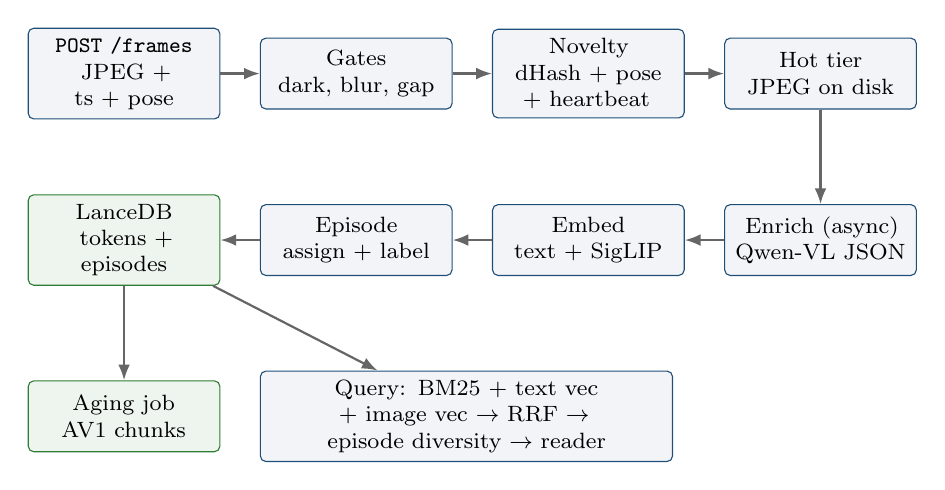
\begin{tikzpicture}[
  box/.style={draw=mmblue,fill=mmblue!6,rounded corners=2pt,minimum height=9mm,text width=22mm,align=center,font=\footnotesize},
  st/.style={draw=mmgreen,fill=mmgreen!8,rounded corners=2pt,minimum height=9mm,text width=22mm,align=center,font=\footnotesize},
  ar/.style={-{Latex[length=2mm]},thick,draw=black!60}, node distance=5mm and 5mm]
\node[box] (in) {\texttt{POST /frames}\\JPEG + ts + pose};
\node[box,right=of in] (gate) {Gates\\dark, blur, gap};
\node[box,right=of gate] (nov) {Novelty\\dHash + pose + heartbeat};
\node[box,right=of nov] (hot) {Hot tier\\JPEG on disk};
\node[box,below=12mm of hot] (enr) {Enrich (async)\\Qwen-VL JSON};
\node[box,left=of enr] (emb) {Embed\\text + SigLIP};
\node[box,left=of emb] (epi) {Episode\\assign + label};
\node[st,left=of epi] (db) {LanceDB\\tokens + episodes};
\node[st,below=12mm of db] (age) {Aging job\\AV1 chunks};
\node[box,right=of age,text width=50mm] (q) {Query: BM25 + text vec + image vec $\rightarrow$ RRF $\rightarrow$ episode diversity $\rightarrow$ reader};
\draw[ar] (in)--(gate); \draw[ar] (gate)--(nov); \draw[ar] (nov)--(hot);
\draw[ar] (hot)--(enr); \draw[ar] (enr)--(emb); \draw[ar] (emb)--(epi); \draw[ar] (epi)--(db);
\draw[ar] (db)--(age); \draw[ar] (db) -- (q);
\end{tikzpicture}
\caption{Stream 1 data flow. Blue: per-frame processing. Green: storage. The request path ends at the hot tier (202 returned); everything below runs asynchronously.}
\end{figure}

\begin{decision}
\textbf{S1 --- The request path stays cheap.} \texttt{POST /frames} only decodes, gates, hashes and writes the JPEG (target $<$ 15\,ms). VLM enrichment, embeddings, episode assignment and aging run in the async worker, so headset upload never blocks on a model.
\end{decision}

% -------------------------------------------------------------------
\section{Filtering}
\subsection{Why the v0.1 filter is not enough}
\begin{measured}
On real camera test footage (1080p, sampled at 1\,fps), a pixel-difference change detector at a camera-tuned threshold kept \textbf{100\%} of frames: sensor noise and head motion mean ``nothing changed'' almost never happens. On screens the same idea dropped 81\% of frames, but at an aggressive threshold it lost 47 of 49 frames of a typing phase and made 2 of 5 questions unanswerable.
\end{measured}
\noindent So the 10--30\% keep rate in v0.1 \S4.2 is unverified, and a pure dHash rule either keeps nearly everything (camera noise) or drops the frame that mattered. The plan: cheap gates, then a novelty score with event triggers, then a per-minute budget.

\subsection{Stages}
\begin{table}[h]\centering\small
\begin{tabular}{P{2.6cm}P{6.4cm}P{2.2cm}P{2.4cm}}\toprule
\textbf{Stage} & \textbf{Rule} & \textbf{Cost} & \textbf{Reason code}\\\midrule
Dark & mean luma $<$ 20 (lens covered, headset off) & $<$1\,ms & \texttt{dark}\\
Blur & variance of Laplacian on 160\,px grey $<$ $\tau_b$ (fast head turns) & $\sim$1\,ms & \texttt{blurry} (new)\\
Min gap & $<$ 2\,s since last kept frame & 0 & \texttt{too\_soon}\\
Novelty & dHash distance to the \emph{last kept} frame and the episode representative; keep if $\ge$ 6 & $<$1\,ms & \texttt{duplicate}\\
Triggers & always keep on: pose change (yaw $>$ 25$^\circ$ or move $>$ 0.75\,m since last kept), heartbeat every 30\,s, client \texttt{force=true} & 0 & ---\\
Budget & token bucket, default 6 kept/min per device; when empty only triggers pass & 0 & \texttt{budget} (new)\\\bottomrule
\end{tabular}
\caption{Filter stages, in order. Thresholds live in \texttt{Settings} and are tuned with the feeder.}
\end{table}

\begin{decision}
\textbf{S2 --- Compare to the last kept frame, not every frame in a 30\,s window.} Comparing against all recent frames lets a slow pan drift forever without a keep; comparing to the last kept frame plus the current episode's representative bounds drift and is O(1).
\end{decision}

\begin{decision}
\textbf{S3 --- Pose is a first-class trigger.} The headset already sends pose; turning to face a new wall or walking into another room is the strongest cheap signal of new content and needs no pixels.
\end{decision}

\subsection{Enrichment budget}
VLM calls are the dominant per-frame cost. The worker enriches a kept frame with Qwen-VL only if it is (a) the first frame of an episode, (b) has SigLIP cosine $<$ 0.92 to the last enriched frame, or (c) is a trigger frame. Other kept frames get an image vector and inherit the episode's caption for BM25, flagged \texttt{enriched=false}; the reader still sees their pixels at query time.
\noindent At 6 kept/min this is $\le$ 360 VLM calls per hour of wear\est.

% -------------------------------------------------------------------
\section{Memory Records}
\subsection{Memory token (additive changes)}
\begin{lstlisting}
MemoryToken {                     # v0.1 fields unchanged
  ...                             # id, device_id, ts, caption, ocr_text, entities,
                                  # pose, text_vec, image_vec, thumb_path, frame_hash
  episode_id: str                 # now filled at ingest (was stretch)
  transcript: str | null          # optional ambient speech overlapping ts
  source: "quest" | "feeder" | "phone"
  trigger: "novel" | "pose" | "heartbeat" | "forced"
  sharpness: float                # Laplacian variance, used for representative choice
  enriched: bool                  # false = caption inherited from episode
  tier: "hot" | "cold" | "text"   # where the pixels live
  chunk_id: str | null            # cold tier: AV1 chunk file
  chunk_offset: int | null        # frame index inside the chunk
}
\end{lstlisting}

\subsection{Memory episode (new table)}
\begin{lstlisting}
MemoryEpisode {
  id, device_id, start_ts, end_ts, n_tokens
  title: str          # zero-shot SigLIP scene label, e.g. "a kitchen"
  summary: str        # optional one-line Qwen/Claude summary when the episode closes
  rep_token_id: str   # sharpest, most-text frame; its JPEG is kept forever
  image_vec: f32[768] # mean of member image vectors (normalised)
  text_vec: f32[d]    # embedding of title + summary + member entities
  pose_centroid: {x,y,z} | null
}
\end{lstlisting}
\noindent New episode when: time gap $>$ 120\,s, or SigLIP cosine of the new frame to the episode representative $<$ 0.80, or pose moves $>$ 3\,m from the centroid. Short detours rejoin one of the last 4 episodes if they match it again within the gap.
\begin{measured}
Image-embedding split threshold 0.80 was calibrated on real screen keyframes: within an episode min 0.83 / median 0.99, across different content 0.73--0.90. It must be re-checked on Quest footage.
\end{measured}

\subsection{Vector sizes}
\begin{table}[h]\centering\small
\begin{tabular}{lrrr}\toprule
\textbf{Vector} & \textbf{dim} & \textbf{fp32} & \textbf{int8}\\\midrule
text, OpenAI \texttt{3-small} & 1536 & 6.0\,KB & 1.5\,KB\\
text, bge-m3 / voyage-3 & 1024 & 4.0\,KB & 1.0\,KB\\
image (SigLIP-base) & 768 & 3.0\,KB & 0.8\,KB\\\bottomrule
\end{tabular}
\caption{Per-token vector cost. Dimensions follow \texttt{EMBED\_PROVIDER}; the LanceDB schema is created from the provider's \texttt{dim}.}
\end{table}

% -------------------------------------------------------------------
\section{Image Storage Tiers}
\begin{table}[h]\centering\small
\begin{tabular}{P{1.6cm}P{3.0cm}P{4.4cm}P{4.4cm}}\toprule
\textbf{Tier} & \textbf{Age} & \textbf{Format} & \textbf{Served as}\\\midrule
Hot & 0--72\,h & JPEG as uploaded (960\,px, q75) & file, \texttt{/v1/thumbs/\{id\}.jpg}\\
Cold & 72\,h -- 100\,d & one AV1 chunk per episode, 960\,px, CRF 50, frame locator per token & decoded on demand, LRU cache, same URL\\
Text & $>$ 100\,d & no pixels except episode representative (WebP) & representative frame\\\bottomrule
\end{tabular}
\caption{Fidelity aging. Text, OCR, captions and vectors are never aged.}
\end{table}

\begin{measured}
Per-frame size on 1080p camera-style test video encoded at 1\,fps: x265 1280 CRF 30: 36--61\,KB; AV1 1280 CRF 50: 6.1--7.6\,KB; AV1 960 CRF 50: 4.4--4.5\,KB. On real screen chunks AV1 at the same width as a good HEVC source came out \emph{larger}, so the cold tier must also choose CRF $\ge$ 50, not only re-quantise.
\end{measured}

\begin{decision}
\textbf{S4 --- Chunk per episode.} Frames within an episode are similar, so inter-frame coding works; an episode is also the unit that is deleted, exported or shown. Kept frames are sparse in time (every $\ge$ 2\,s), so expect up to 2$\times$ the consecutive-frame size\est: $\sim$9\,KB per frame.
\end{decision}

\subsection{Storage budget}
\begin{table}[h]\centering\small
\begin{tabular}{P{4.3cm}rrr}\toprule
 & \textbf{Default budget} & \textbf{30\% keep} & \textbf{100\% keep}\\\midrule
Kept frames per 16\,h day & 5\,760 & 17\,280 & 57\,600\\
Hot JPEG, 3 days (100\,KB\est) & 1.7\,GB & 5.2\,GB & 17\,GB\\
Cold AV1, 100 days (9\,KB\est) & 5.2\,GB & 16\,GB & 52\,GB\\
Vectors, 100 days, int8 (2.3\,KB) & 1.3\,GB & 4.0\,GB & 13\,GB\\
Text + metadata, 100 days (1\,KB) & 0.6\,GB & 1.7\,GB & 5.8\,GB\\\midrule
\textbf{Total for 100 days} & \textbf{$\approx$ 9\,GB} & \textbf{$\approx$ 27\,GB} & \textbf{$\approx$ 88\,GB}\\\bottomrule
\end{tabular}
\caption{Estimated storage for 100 days of 16\,h wear (sampling 1\,fps). Replace the \est{} figures with feeder measurements on hour 3.}
\end{table}

% -------------------------------------------------------------------
\section{Retrieval}
\subsection{Store layout (LanceDB)}
\begin{itemize}
  \item \texttt{tokens}: all MemoryToken columns; vector columns \texttt{text\_vec}, \texttt{image\_vec}; FTS index on \texttt{caption}, \texttt{ocr\_text}, \texttt{entities\_text}, \texttt{transcript}; scalar index on \texttt{ts}, \texttt{device\_id}, \texttt{episode\_id}.
  \item \texttt{episodes}: MemoryEpisode; vector columns; FTS on \texttt{title}, \texttt{summary}.
  \item The existing \texttt{InMemoryStore} stays as the test double and gets the same fusion code.
\end{itemize}

\subsection{Query pipeline}
\begin{enumerate}
  \item \textbf{Filter:} device and time range (Claude passes ISO bounds; a regex fallback parses ``at 3\,pm'', ``this morning'', ``20 minutes ago'' for \texttt{GET /memories}).
  \item \textbf{Retrieve} top 50 from each: BM25 (AND of terms, fall back to OR), text-vector cosine, SigLIP text$\rightarrow$image cosine.
  \item \textbf{Fuse} with weighted RRF: $\;s(t)=\sum_r w_r/(60+\mathrm{rank}_r(t))$, $w_\text{bm25}=w_\text{text}=1.0$, $w_\text{image}=0.6$ (\texttt{visual} mode: 1.5).
  \item \textbf{Diversify:} at most 3 tokens per episode in the top $k$.
  \item \textbf{Expand:} attach the episode title and the $\pm$30\,s neighbours' captions as context lines.
  \item \textbf{Pack for the reader:} episode representatives first, then top tokens; for OCR questions send a high-resolution crop around the text instead of the downscaled frame.
\end{enumerate}
\begin{measured}
On the screenmem 16-question gold set: BM25 hit@1 87.5\%, hit@5 93.8\%; dense text hit@1 68.8\%, hit@5 100\%; their union reached 100\% hit@5. A glasses-style gold set with visual-only and speech questions reached 8/8 hit@1 with three-signal fusion. These are small sets.
\end{measured}

\subsection{Activity questions}
\texttt{GET /v1/episodes?from=\&to=\&q=} returns episodes in time order, ranked by the summed fused score of their tokens when \texttt{q} is given. Claude gets a second tool, \texttt{list\_episodes(time\_from, time\_to, query?)}, so ``what did I do after lunch'' is one call returning 5--20 compact lines instead of 24 frames.

% -------------------------------------------------------------------
\section{Contract Changes}
All additive; one PR updates \texttt{docs/api.md}, \texttt{models.py} and \texttt{Dto.cs} together, per the integration rule.
\begin{table}[h]\centering\small
\begin{tabular}{P{4.2cm}P{9.8cm}}\toprule
\textbf{Change} & \textbf{Effect on headset}\\\midrule
\texttt{reason} gains \texttt{blurry}, \texttt{budget} & none (status HUD can show it)\\
optional \texttt{meta.force}, \texttt{meta.source} & optional; \texttt{force} on push-to-talk start keeps the frame the user is looking at\\
\texttt{MemoryHit} gains \texttt{episode\_id}, \texttt{episode\_title}, \texttt{tier} & none\\
new \texttt{GET /v1/episodes} & optional timeline panel\\
new tool \texttt{list\_episodes} & none (server-side)\\\bottomrule
\end{tabular}
\end{table}

% -------------------------------------------------------------------
\section{Evaluation}
\begin{itemize}
  \item \textbf{Fixture:} 20--30 minute walkthrough video (keys on counter, whiteboard, poster, person talking) fed with \texttt{tools/feeder.py --realtime}; also the public test clips used in screenmem.
  \item \textbf{Gold set:} JSON of \texttt{\{q, expect\_substrings | expect\_token\_ids | expect\_episodes, time?\}}; \texttt{tools/eval.py} reports hit@1, hit@5, mean latency.
  \item \textbf{Efficiency report:} \texttt{GET /v1/stats}: keep rate per reason, VLM calls/hour, bytes per tier, projected GB per 100 days.
  \item \textbf{CI:} mock embedders and a synthetic image fixture test filter decisions, fusion order, episode splits and aging round-trip (encode $\rightarrow$ decode a frame by locator).
\end{itemize}

% -------------------------------------------------------------------
\section{Work Plan}
\begin{table}[h]\centering\small
\begin{tabular}{rP{6.2cm}rP{5.0cm}}\toprule
\# & \textbf{Task} & \textbf{h\est} & \textbf{Done when}\\\midrule
1 & Filter v2: blur, last-kept novelty, pose + heartbeat triggers, budget & 1.5 & unit tests; feeder keep-rate printed\\
2 & Real embedders: OpenAI/Voyage text, local SigLIP image + text tower & 1.5 & \texttt{EMBED\_PROVIDER} switch works\\
3 & Qwen-VL enricher (JSON prompt, Claude Haiku fallback) + enrichment budget & 1.0 & captions on feeder frames\\
4 & LanceDBStore: schema, FTS, vector search, weighted RRF, diversity & 2.5 & same tests pass on both stores\\
5 & Episodes: assign, scene label, representative, \texttt{/v1/episodes}, \texttt{list\_episodes} & 2.0 & ``what did I do'' returns ordered episodes\\
6 & Aging: AV1 chunk per episode, locator, on-demand decode, delete & 2.0 & round-trip test; \texttt{/thumbs} serves cold frames\\
7 & Eval + stats: gold set runner, \texttt{/v1/stats}, fixture video & 1.5 & hit@5 and GB/100\,d on dashboard\\\midrule
 & \textbf{Total} & \textbf{12} & \\\bottomrule
\end{tabular}
\end{table}
\noindent Order: 1 $\rightarrow$ 2 $\rightarrow$ 4 gives a queryable vertical slice; 3, 5, 6, 7 follow. Tasks 6 and 7 can run in parallel with others.

% -------------------------------------------------------------------
\section{Risks}
\begin{risk}
\textbf{Keep rate on real passthrough is unknown.} Mitigation: the budget caps it regardless; feeder measurement on hour 3 sets thresholds.
\end{risk}
\begin{risk}
\textbf{VLM enrichment latency or cost.} Mitigation: enrichment budget (\S3.3), queue drop-oldest, image-vector-only tokens stay searchable visually.
\end{risk}
\begin{risk}
\textbf{SigLIP on CPU is slow.} Mitigation: batch in the worker; base model at 224\,px is $\sim$50--100\,ms per image on a laptop CPU\est; GPU if available.
\end{risk}
\begin{risk}
\textbf{Bystander privacy.} Mitigation: no identity prompts, local storage, purge by device and by time range, capture indicator on the HUD.
\end{risk}

\end{document}
